

\tikzset{every picture/.style={line width=0.75pt}} %set default line width to 0.75pt        

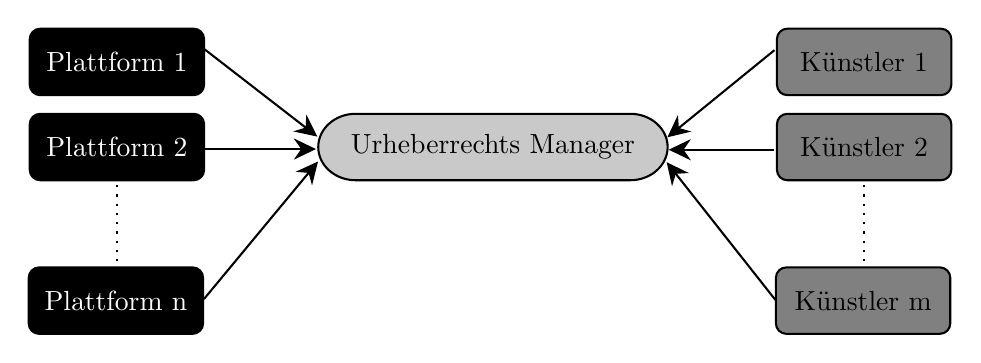
\begin{tikzpicture}[x=0.75pt,y=0.75pt,yscale=-1,xscale=1]
%uncomment if require: \path (0,385.23333740234375); %set diagram left start at 0, and has height of 385.23333740234375

%Shape: Rectangle [id:dp629393056464483] 
\draw  [color={rgb, 255:red, 0; green, 0; blue, 0 }  ,draw opacity=1 ][fill={rgb, 255:red, 0; green, 0; blue, 0 }  ,fill opacity=1 ] (100,6) .. controls (100,3.24) and (102.24,1) .. (105,1) -- (179,1) .. controls (181.76,1) and (184,3.24) .. (184,6) -- (184,28) .. controls (184,30.76) and (181.76,33) .. (179,33) -- (105,33) .. controls (102.24,33) and (100,30.76) .. (100,28) -- cycle ;
%Shape: Rectangle [id:dp7576997309692058] 
\draw  [fill={rgb, 255:red, 0; green, 0; blue, 0 }  ,fill opacity=1 ] (100,47) .. controls (100,44.24) and (102.24,42) .. (105,42) -- (179,42) .. controls (181.76,42) and (184,44.24) .. (184,47) -- (184,69) .. controls (184,71.76) and (181.76,74) .. (179,74) -- (105,74) .. controls (102.24,74) and (100,71.76) .. (100,69) -- cycle ;
%Shape: Rectangle [id:dp11064096186910266] 
\draw  [fill={rgb, 255:red, 0; green, 0; blue, 0 }  ,fill opacity=1 ] (99.5,121) .. controls (99.5,118.24) and (101.74,116) .. (104.5,116) -- (178.5,116) .. controls (181.26,116) and (183.5,118.24) .. (183.5,121) -- (183.5,143) .. controls (183.5,145.76) and (181.26,148) .. (178.5,148) -- (104.5,148) .. controls (101.74,148) and (99.5,145.76) .. (99.5,143) -- cycle ;
%Straight Lines [id:da665164617841208] 
\draw  [dash pattern={on 0.84pt off 2.51pt}]  (141.87,76.29) -- (141.87,116.23) ;


%Shape: Rectangle [id:dp06887041087701307] 
\draw  [fill={rgb, 255:red, 201; green, 201; blue, 201 }  ,fill opacity=1 ] (239,58) .. controls (239,49.16) and (247.06,42) .. (257,42) -- (389.33,42) .. controls (399.27,42) and (407.33,49.16) .. (407.33,58) .. controls (407.33,66.84) and (399.27,74) .. (389.33,74) -- (257,74) .. controls (247.06,74) and (239,66.84) .. (239,58) -- cycle ;
%Shape: Rectangle [id:dp999529442839202] 
\draw  [fill={rgb, 255:red, 128; green, 128; blue, 128 }  ,fill opacity=1 ] (460,6) .. controls (460,3.24) and (462.24,1) .. (465,1) -- (539,1) .. controls (541.76,1) and (544,3.24) .. (544,6) -- (544,28) .. controls (544,30.76) and (541.76,33) .. (539,33) -- (465,33) .. controls (462.24,33) and (460,30.76) .. (460,28) -- cycle ;
%Shape: Rectangle [id:dp039134238266278376] 
\draw  [fill={rgb, 255:red, 128; green, 128; blue, 128 }  ,fill opacity=1 ] (460,47) .. controls (460,44.24) and (462.24,42) .. (465,42) -- (539,42) .. controls (541.76,42) and (544,44.24) .. (544,47) -- (544,69) .. controls (544,71.76) and (541.76,74) .. (539,74) -- (465,74) .. controls (462.24,74) and (460,71.76) .. (460,69) -- cycle ;
%Shape: Rectangle [id:dp7280368044947276] 
\draw  [fill={rgb, 255:red, 128; green, 128; blue, 128 }  ,fill opacity=1 ] (459.5,121) .. controls (459.5,118.24) and (461.74,116) .. (464.5,116) -- (538.5,116) .. controls (541.26,116) and (543.5,118.24) .. (543.5,121) -- (543.5,143) .. controls (543.5,145.76) and (541.26,148) .. (538.5,148) -- (464.5,148) .. controls (461.74,148) and (459.5,145.76) .. (459.5,143) -- cycle ;
%Straight Lines [id:da4054781940287375] 
\draw  [dash pattern={on 0.84pt off 2.51pt}]  (501.87,76.29) -- (501.87,116.23) ;


%Straight Lines [id:da2213724342070541] 
\draw    (184.33,11) -- (236.97,51.75) ;
\draw [shift={(238.56,52.98)}, rotate = 217.75] [fill={rgb, 255:red, 0; green, 0; blue, 0 }  ][line width=0.75]  [draw opacity=0] (10.72,-5.15) -- (0,0) -- (10.72,5.15) -- (7.12,0) -- cycle    ;

%Straight Lines [id:da6616664886016944] 
\draw    (184.56,58.98) -- (235.89,58.98) ;
\draw [shift={(237.89,58.98)}, rotate = 180] [fill={rgb, 255:red, 0; green, 0; blue, 0 }  ][line width=0.75]  [draw opacity=0] (10.72,-5.15) -- (0,0) -- (10.72,5.15) -- (7.12,0) -- cycle    ;

%Straight Lines [id:da07563821279207716] 
\draw    (183.89,131.31) -- (237.61,66.52) ;
\draw [shift={(238.89,64.98)}, rotate = 489.66] [fill={rgb, 255:red, 0; green, 0; blue, 0 }  ][line width=0.75]  [draw opacity=0] (10.72,-5.15) -- (0,0) -- (10.72,5.15) -- (7.12,0) -- cycle    ;

%Straight Lines [id:da19634229810211157] 
\draw    (458.8,11.33) -- (408.77,52.05) ;
\draw [shift={(407.22,53.31)}, rotate = 320.86] [fill={rgb, 255:red, 0; green, 0; blue, 0 }  ][line width=0.75]  [draw opacity=0] (10.72,-5.15) -- (0,0) -- (10.72,5.15) -- (7.12,0) -- cycle    ;

%Straight Lines [id:da21586829986315392] 
\draw    (458.59,59.31) -- (409.86,59.31) ;
\draw [shift={(407.86,59.31)}, rotate = 360] [fill={rgb, 255:red, 0; green, 0; blue, 0 }  ][line width=0.75]  [draw opacity=0] (10.72,-5.15) -- (0,0) -- (10.72,5.15) -- (7.12,0) -- cycle    ;

%Straight Lines [id:da5626991905148753] 
\draw    (459.22,131.64) -- (408.1,66.88) ;
\draw [shift={(406.86,65.31)}, rotate = 411.71000000000004] [fill={rgb, 255:red, 0; green, 0; blue, 0 }  ][line width=0.75]  [draw opacity=0] (10.72,-5.15) -- (0,0) -- (10.72,5.15) -- (7.12,0) -- cycle    ;


% Text Node
\draw (142,17) node [color={rgb, 255:red, 255; green, 255; blue, 255 }  ,opacity=1 ] [align=left] {Plattform 1};
% Text Node
\draw (142,58) node [color={rgb, 255:red, 255; green, 255; blue, 255 }  ,opacity=1 ] [align=left] {Plattform 2};
% Text Node
\draw (141.5,132) node [color={rgb, 255:red, 255; green, 255; blue, 255 }  ,opacity=1 ] [align=left] {Plattform n};
% Text Node
\draw (323.17,58) node [color={rgb, 255:red, 0; green, 0; blue, 0 }  ,opacity=1 ] [align=left] {Urheberrechts Manager};
% Text Node
\draw (502,17) node  [align=left] {Künstler 1};
% Text Node
\draw (502,58) node  [align=left] {Künstler 2};
% Text Node
\draw (501.5,132) node  [align=left] {Künstler m};


\end{tikzpicture}
